\section{Manuel utilisateur}
\label{sec:manuel}

Bienvenue dans le manuel utilisateur de Glasir, un logiciel d'aide aux experts en sécurité basé sur le formalisme des ADTrees\footnote{Abréviation d'\og Attack-Defense Trees \fg{}, ou \og Arbres d'Attaque et de Défense\fg{} en français.}. Grâce à Glasir, vous pourrez analyser efficacement vos ADTrees préalablement créés avec ADTool~\cite{adtool}, un logiciel open-source disponible sur Internet.

Ce livret commencera par décrire le fonctionnement général du logiciel (création d'un nouveau projet, ouverture d'un projet existant, etc.), avant d'expliquer comment prendre en main les trois fonctionnalités principales que sont l'Éditeur de fonctions, le Filtre et enfin l'Optimiseur. 

Après cela, dans la {\sc sous-section}~\ref{ssec:manuelADTool} vous trouverez des détails concernant l'utilisation d'ADTool, surtout les nouveautés qui lui ont été ajoutées lors de ce projet.

\begin{figure}[!h]
        \centering
        
\includegraphics[height=0.3\textwidth]{figure/glasir.png}
        \caption{Logo du logiciel Glasir.}
    \end{figure}

\subsection{Glasir}
\label{ssec:manuelGlasir}

\paragraph{Fonctionnement général}

\paragraph{Éditeur de fonctions}

\paragraph{Filtre}

\paragraph{Optimiseur}

\subsection{Nouvelles fonctionnalités d'ADTool}
\label{ssec:manuelADTool}

Pour le fonctionnement basique d'ADTool, vous pouvez vous référer au manuel utilisateur officiel disponible sur Internet\footnote{Voir à l'adresse suivante : http://satoss.uni.lu/members/piotr/adtool/manual.pdf}. Le guide ici présent ne détaillera que l'utilisation des nouvelles fonctionnalités d'ADTool, qui sont le copier/couper/coller ainsi que l'annulation d'une action.

\paragraph{Copier/couper/coller} Ces fonctionnalités vous seront utiles si vous désirez couper/copier un sous-arbre de l'ADTree courant afin de le coller ensuite à un autre emplacement dans ce même ADTree. Il est à noter que le sous-arbre coupé/copié sera ajouté en tant que fils du n\oe{}ud auquel il sera collé. Aussi, la racine du sous-arbre coupé/copié doit être du même type (opponent ou proponent) que son futur n\oe{}ud parent. Pour couper/copier un sous-arbre puis le coller, suivez les étapes suivantes : 
\begin{enumerate}
    \item Sélectionnez à l'aide d'un clic gauche le n\oe{}ud racine du sous-arbre que vous désirez couper/copier. Si vous avez déjà sélectionné un n\oe{}ud dans l'arbre, vous pouvez également vous déplacer jusqu'au n\oe{}ud souhaité à l'aide des flèches (haut, bas, gauche, droite) du clavier.
	\item Effectuez un clic droit sur le n\oe{}ud sélectionné. Un menu déroulant doit apparaître à côté du n\oe{}ud sélectionné, comme sur la {\sc Figure}~\ref{fig:clicdroit}.
	\item Sélectionnez l'option \og Copy Subtree \fg{}/\og Cut Subtree \fg{}) dans le menu déroulant. Vous pouvez également effectuer cette étape à l'aide d'un raccourci clavier, {\sc CTRL+C}/{\sc CTRL+X}.
	\item Effectuez un clic droit sur le n\oe{}ud auquel vous voulez coller le sous-arbre coupé/copié, puis sélectionnez dans la liste déroulante \og Paste Subtree as Child \fg{}. Si cette option n'apparaît pas dans le menu déroulant, c'est que vous n'avez pas préalablement coupé/copié de sous-arbre. Vous pouvez ici encore utiliser un raccourci clavier, {\sc CTRL+V}.
\end{enumerate}

    \begin{figure}[!h]
        \centering
        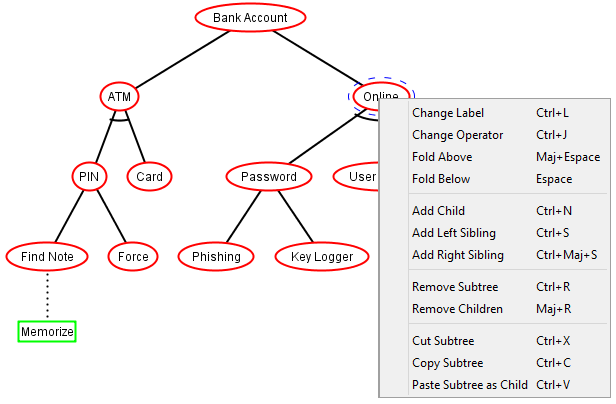
\includegraphics[height=0.7\textwidth]{figure/clicdroit.png}
        \caption{Menu déroulant apparaissant après un clic droit sur un n\oe{}ud.}
        \label{fig:clicdroit}
    \end{figure}

\paragraph{Annulation d'une action} Il s'agit ici d'annuler une ou plusieurs action(s) effectuée(s) précédemment sur l'ADTree courant. Pour cela, il vous suffit tout simplement d'utiliser le raccourci clavier {\sc CTRL+Z} autant de fois que nécessaire, jusqu'à retrouver l'état souhaité pour l'ADTree. Vous pouvez également cliquer sur l'icône \og Undo last action (CTRL+Z) \fg{} en haut à gauche de la fenêtre principale d'ADTool, encadrée en rouge sur la {\sc figure}~\ref{fig:undo}. Les actions pouvant être annulées sont les changements de labels, les ajouts ou suppressions de n\oe{}uds, les changements d'opérateur (conjonction ou disjonction) ainsi que les actions de couper/copier/coller.

\begin{figure}[!h]
        \centering
        
\includegraphics[height=0.17\textwidth]{figure/undo.png}
        \caption{Icône permettant d'annuler l'action précédente.}
        \label{fig:undo}
    \end{figure}